%!TEX root = ../../Master.tex
\section{Organization} % (fold)
\label{sec:organization}


In order to create a good navigational system for a hospital, certain factors must be considered. When deciding new features for a hospital, installation \& maintenance costs and compatibility with the existing hardware are big subjects. Therefore this section will describe how the existing infrastructure in hospitals is and how this will affect the navigational system.


In order to create a good navigational system for a hospital, certain factors must be considered. When deciding new features for a hospital, installation \& maintenance costs and compatibility with the existing hardware are big subjects. Therefore this section will describe how the existing infrastructure in hospitals is, and how this will affect the navigational system.

\subsection{WiFi} \label{orgwifi}

Most hospitals have good WiFi coverage around their cadastral. A visit to \enquote{Sygehus Nord} in Aalborg revealed that multiple locations around the hospital had a sufficient amount of WiFi hotspots in range, in order to be used in Location Based Services. See \cref{fig:wifi1,fig:wifi2,fig:wifi3}.

\begin{figure}
\centering
  \begin{minipage}{0.45\textwidth}
    \centering
    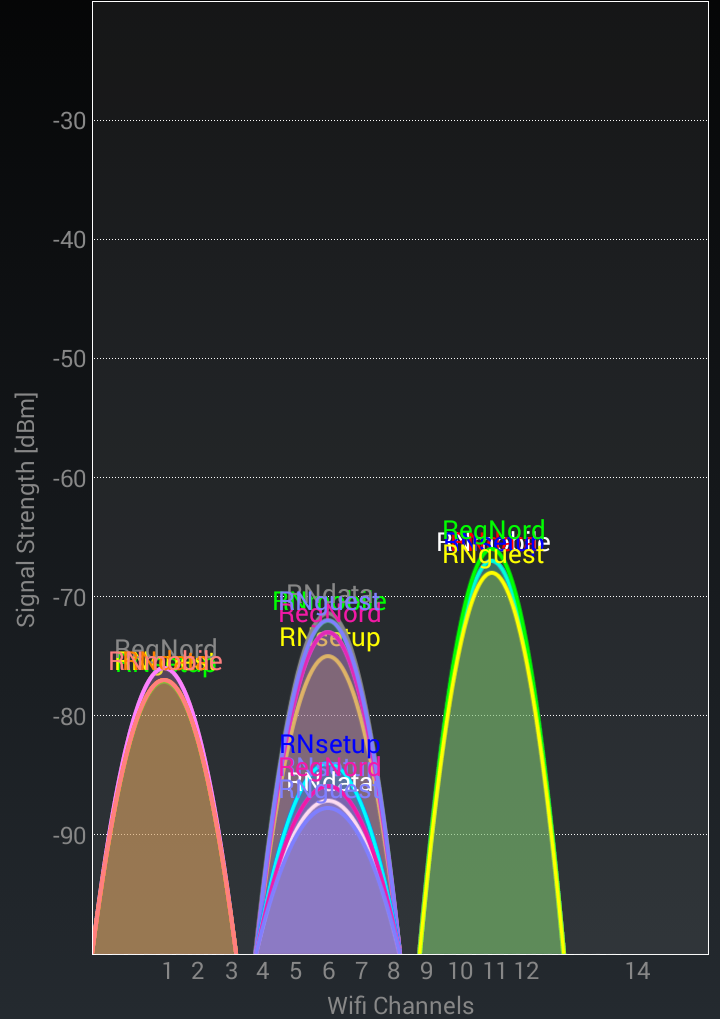
\includegraphics[width=\textwidth]{wifi_sygehus_nord1.png}
    \caption{Graph of signal strength grouped by channels. Location A} \label{fig:wifi1}
  \end{minipage}
  \hfill
  \begin{minipage}{0.45\textwidth}
    \centering
    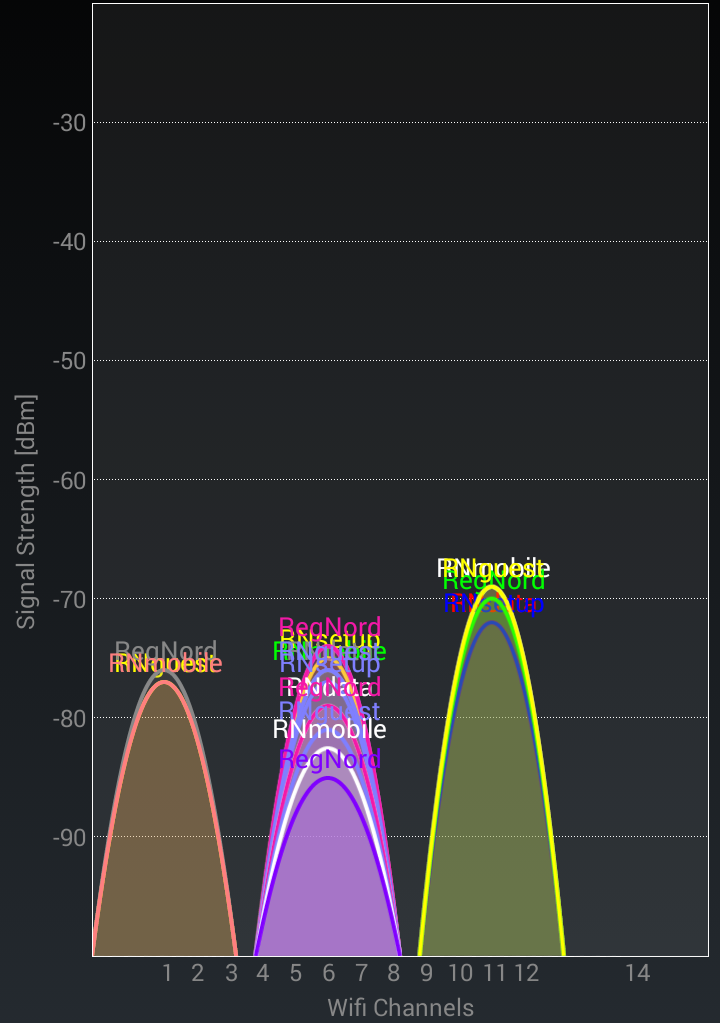
\includegraphics[width=\textwidth]{wifi_sygehus_nord2.png}
    \caption{Graph of signal strength grouped by channels. Location B} \label{fig:wifi2}
  \end{minipage}
    \begin{minipage}{0.45\textwidth}
    \centering
    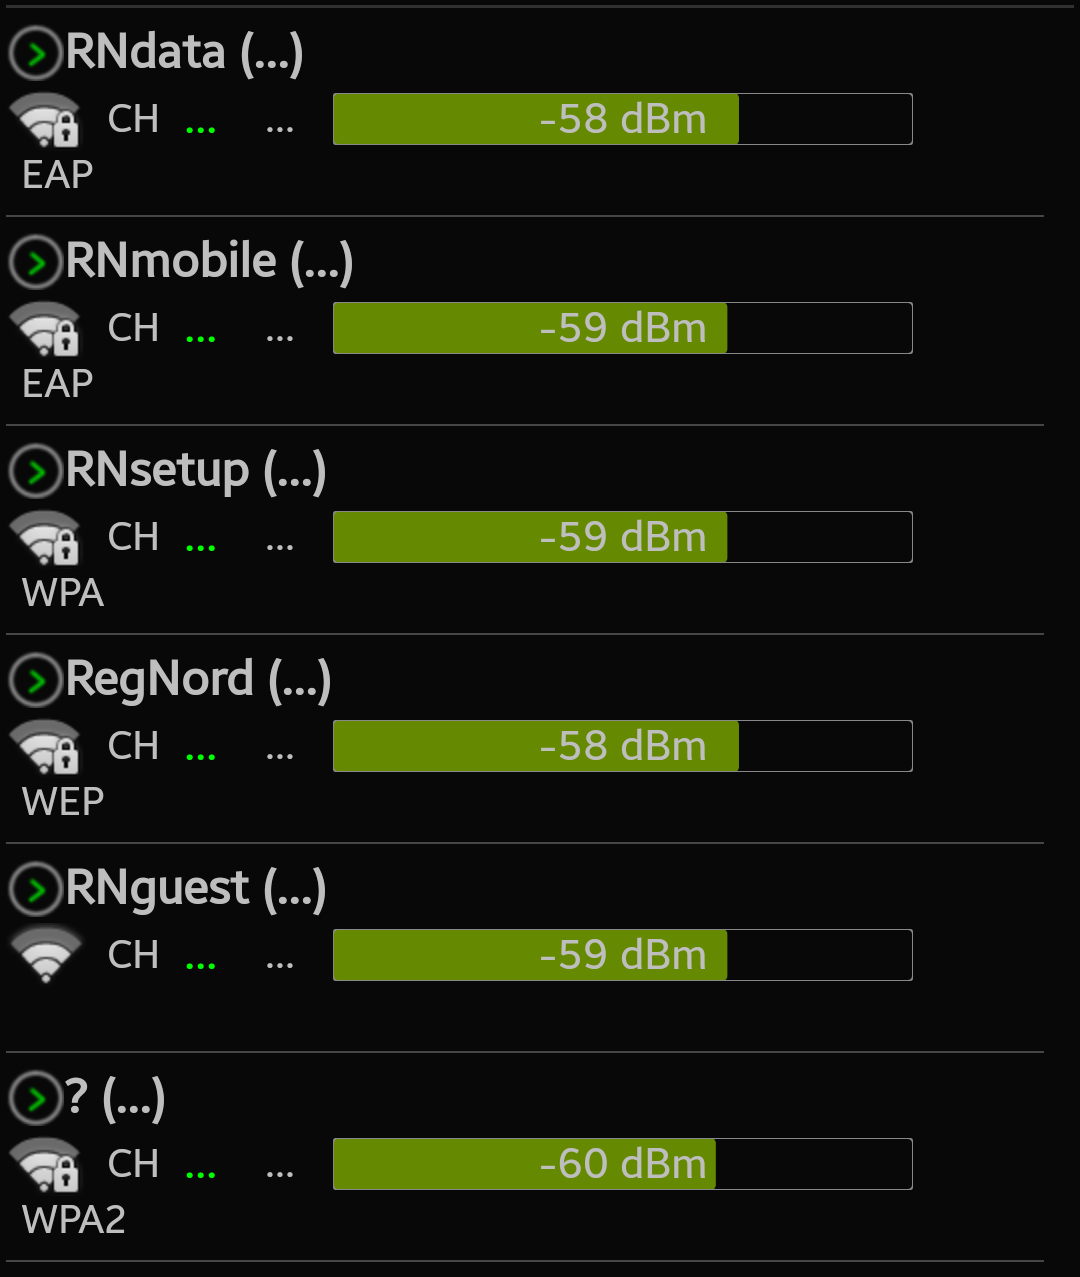
\includegraphics[width=\textwidth]{wifi_sygehus_nord3.png}
    \caption{List of WiFi networks} \label{fig:wifi3}
  \end{minipage}
  \end{figure}


\subsection{Interference with medical device}

Incidents of radio frequency interference between cellular phones, radio broadcasters, WiFi devices and medical devices have been reported. Older models of pacemakers, defibrillators and hearing aid devices were being influenced by near encounter of cellular phones causing undesirable effects like not having control of heartbeat etc. 
The problem was that radio frequency fields were interfering with medical equipment. This has however now been addressed in modern standards, meaning that interference with medical devices does not occur any more. \cite{Man1998,Case}

\subsection{Temporary out-of-order elements}

When mapping a hospital every hall building, stair, elevator etc. has to be considered. Situations may however occur in which some of the mapped elements in fact are temporary out-of-order. This could be an elevator or a hallway being repainted. Updating the navigation system map to include the temporary elements could be a lot of effort. In a situation in which an user of the navigation system is guided through an out-of-order element, the user will most likely find their own way around this obstacle. When this happens, the user is going off-route. The navigation system must support this and act accordingly.


\subsection{Cross-building support}

Some hospitals will undoubtedly have several building complexes around their cadastral. A good navigational system should work across these platforms providing one, uniform experience. This is both good for the end-user, but as the navigational system can be reused also eases the installation. If support for cross-building complexes has been laid, this could further expand to the navigation system supporting different hospitals independent of each other. The navigation system could then e.g. be installed in all the hospitals in Region Nord, providing an uniform experience for end-users.


% section organization (end)